\documentclass[
  bibliography=totoc,     % Literatur im Inhaltsverzeichnis
  captions=tableheading,  % Tabellenüberschriften
  titlepage=firstiscover, % Titelseite ist Deckblatt
]{scrartcl}

% Vektoren
\usepackage{esvect}


% Paket float verbessern
\usepackage{scrhack}

% Warnung, falls nochmal kompiliert werden muss
\usepackage[aux]{rerunfilecheck}

% unverzichtbare Mathe-Befehle
\usepackage{amsmath}
% viele Mathe-Symbole
\usepackage{amssymb}
% Erweiterungen für amsmath
\usepackage{mathtools}

% Fonteinstellungen
\usepackage{fontspec}
% Latin Modern Fonts werden automatisch geladen
% Alternativ zum Beispiel:
%\setromanfont{Libertinus Serif}
%\setsansfont{Libertinus Sans}
%\setmonofont{Libertinus Mono}

% Wenn man andere Schriftarten gesetzt hat,
% sollte man das Seiten-Layout neu berechnen lassen
\recalctypearea{}

% deutsche Spracheinstellungen
\usepackage{polyglossia}
\setmainlanguage{german}

% Blindtext
\usepackage{blindtext}

\usepackage[
  math-style=ISO,    % ┐
  bold-style=ISO,    % │
  sans-style=italic, % │ ISO-Standard folgen
  nabla=upright,     % │
  partial=upright,   % ┘
  warnings-off={           % ┐
    mathtools-colon,       % │ unnötige Warnungen ausschalten
    mathtools-overbracket, % │
  },                       % ┘
]{unicode-math}

% traditionelle Fonts für Mathematik
\setmathfont{Latin Modern Math}
% Alternativ zum Beispiel:
%\setmathfont{Libertinus Math}

\setmathfont{XITS Math}[range={scr, bfscr}]
\setmathfont{XITS Math}[range={cal, bfcal}, StylisticSet=1]

% Zahlen und Einheiten
\usepackage[
  locale=DE,                   % deutsche Einstellungen
  separate-uncertainty=true,   % immer Fehler mit \pm
  per-mode=symbol-or-fraction, % / in inline math, fraction in display math
]{siunitx}

% chemische Formeln
\usepackage[
  version=4,
  math-greek=default, % ┐ mit unicode-math zusammenarbeiten
  text-greek=default, % ┘
]{mhchem}

% richtige Anführungszeichen
\usepackage[autostyle]{csquotes}

% schöne Brüche im Text
\usepackage{xfrac}
\usepackage{nicefrac}

% Standardplatzierung für Floats einstellen
\usepackage{float}
\floatplacement{figure}{htbp}
\floatplacement{table}{htbp}

% Floats innerhalb einer Section halten
\usepackage[
  section, % Floats innerhalb der Section halten
  below,   % unterhalb der Section aber auf der selben Seite ist ok
]{placeins}

% Seite drehen für breite Tabellen: landscape Umgebung
\usepackage{pdflscape}

% Captions schöner machen.
\usepackage[
  labelfont=bf,        % Tabelle x: Abbildung y: ist jetzt fett
  font=small,          % Schrift etwas kleiner als Dokument
  width=0.9\textwidth, % maximale Breite einer Caption schmaler
]{caption}
% subfigure, subtable, subref
\usepackage{subcaption}

% Grafiken können eingebunden werden
\usepackage{graphicx}
% größere Variation von Dateinamen möglich
\usepackage{grffile}

% schöne Tabellen
\usepackage{booktabs}

% Verbesserungen am Schriftbild
\usepackage{microtype}

% Literaturverzeichnis
\usepackage[
  backend=biber,
]{biblatex}
% Quellendatenbank
\addbibresource{lit.bib}
\addbibresource{programme.bib}

% Hyperlinks im Dokument
\usepackage[
  unicode,        % Unicode in PDF-Attributen erlauben
  pdfusetitle,    % Titel, Autoren und Datum als PDF-Attribute
  pdfcreator={},  % ┐ PDF-Attribute säubern
  pdfproducer={}, % ┘
]{hyperref}
% erweiterte Bookmarks im PDF
\usepackage{bookmark}

% Trennung von Wörtern mit Strichen
\usepackage[shortcuts]{extdash}
%Erlaubt Einfügen von PDF-Dateien
\usepackage{pdfpages}
\author{%
  Lars Kolk\\%
  \href{mailto:lars.kolk@tu-dortmund.de}{lars.kolk@tu-dortmund.de}%
  \texorpdfstring{\and}{,}%
  Julia Sobolewski\\%
  \href{mailto:julia.sobolewski@tu-dortmund.de}{julia.sobolewski@tu-dortmund.de}%
  \texorpdfstring{\and}{,}%
  Jannine Salewski\\%
  \href{mailto:Jannine.salewski@tu-dortmund.de}{jannine.salewski@tu-dortmund.de}%
}
\publishers{TU Dortmund – Fakultät Physik}

\usepackage{longtable}
\usepackage{wrapfig}
\usepackage{ dsfont }
\usepackage{tcolorbox}
\subject{SMD-Abgabe}
\title{9. Übungsblatt}
\date{%
  Abgabe: 20.12.2018
}

\begin{document}
  \setlength{\parindent}{0em}
  \maketitle
  \thispagestyle{empty}
  \newpage
  %\tableofcontents
  %\newpage

  \newenvironment{console1}[1]
  {\begin{center}
  \begin{minipage}[t]{0.99\linewidth}
  \begin{tcolorbox}[colback=gray!5,colframe=black!40!black,title= Ausgabe des Programms: #1 ]
    }
    {
  \end{tcolorbox}
  \end{minipage}
  \end{center}
  }

%\paragraph{Aufgabe 17}


\subparagraph{a)}
Nicht-numerische Datentypen sollten, wenn möglich (und sinnvoll), in Zahlen ausgedrückt werden um mit ihnen besser arbeiten zu können.
Im Fall der Titanic könnte z.B. der Status der Passagiere (also ob tot oder lebendig) als 0 oder 1 dargestellt werden.
Sollte es jedoch nicht-numerische Datentypen geben, die sich nicht sinnvoll in Zahlen ausdrücken lassen, könnte man diese verfallen lassen, sofern sie für die Untersuchung irrelevant sind.
Ebenso könnte man dann mit nicht-numerische Datentypen weiterarbeiten, sofern dies die Aufbereitung des Datensatzes nicht erschwert.

\subparagraph{b)}
Die normierung der Attribute kann sinnvoll sein, da Attribute bei verschiedenen Größenordnungen verschieden gewichtet sein können.
Dadurch könnte einigen Attributen mehr Bedeutung als anderen zugemessen werden, obwohl die Größenordnung nicht ausschlaggebend für die Wichtigkeit ist. Dem kann durch Normierung vorgebeugt werden.
\subparagraph{c)}
Sofern nur wenige Daten des Datensatzes Lücken aufweisen, können diese ggf. verworfen werden. Das ist jedoch auch vom zu untersuchenden Datensatz abhängig, da auch fehlende Informationen Informationen sind.
Wenn die betroffenden Daten dennoch in die Untersuchung eingehen oder seperat auf Korrelation mit ihren Attributen untersucht werden sollen, kann es sinnvoll sein, die Lücken einheitlich zu füllen (z.B. alles auf NaN setzen).

\subparagraph{d)}
Die Datensätze sollten vom selben Typ sein. Ebenso könnte es sinnvoll sein, die Datensätze vor dem zusammenfügen entsprechend zu labeln, sodass durch das Zusammenfügen keine Informationen verloren gehen.

\subparagraph{e)}
Redudante Attribute sind vor dem Trainieren der Klassifizierers zu entfernen. Dies kann z.B. per Hand, aber auch durch Entscheidungsbäume geschehen, die einen günstige Schnitt mit mit einem hohen informationsgehalt finden. 

%\paragraph{18}
\subparagraph{a}
Mit der bedingten Wahrscheinlichkeit folgt:
\begin{equation}
P(F|W) = \frac{P(F\cap\ W)}{P(W)} = \frac{\frac{P(F\,\cap\, W)}{P(F)}\cdot P(F)}{P(W)} = \frac{P(W|F)\cdot P(F)}{P(W)}
\end{equation}

\subparagraph{b)}
Mit
\begin{equation}
  P(F)=9/14
\end{equation}
folgt mit der Wahrscheinlichkeit der gesuchten Attributen in $F$
\begin{align}
%Wahrscheinlichkeit für die geg. Parameter in F:
P_{Wind_F}=\frac{1}{3} \\
P_{Temp_F}=\frac{1}{3} \\
P_{Feucht_F}=\frac{1}{3} \\
P_{Aussicht_F}=\frac{2}{9}
\end{align}
und mit der Gesamtwahrscheinlichkeit der Ereignisse
\begin{align}
  P_{Wind_{Stark}}=\frac{6}{14} \\
  P_{Temp_{Kalt}}=\frac{6}{14} \\
  P_{Aussicht_{Sonnig}}=\frac{3}{14} \\
  P_{Feucht_{Hoch}}=\frac{7}{14} \\
\end{align}
und dem in der Aufgabenstellung gegebenen Zusammenhang
\begin{equation}
  P(F| W)=\prod_{i} P(x_i | W)
\end{equation} der Zusammenhang
\begin{align}
  P(F | W) =& \frac{P_{Wind_F} \cdot P_{Temp_F} \cdot P_{Feucht_F} \cdot P_{Aussicht_F}\cdot P(F)}{P_{Wind_{Stark}} \cdot P_{Temp_{Kalt}} \cdot P_{Aussicht_{Sonnig}} \cdot P_{Feucht_{Hoch}}} \\
  P(F | W) =& 26,9 \%
\end{align}
.

\subparagraph{c)}
Die Wahrscheinlichkeit beträgt 0, da der Datensatz keine Aufzeichnungen von stattgefundenden Spielen bei heißen Temperaturen enthält.
Dies erzeugt einen Faktor 0, der das gesamte Produkt 0 werden lässt.
Ein größerer Datensatz könnte das Problem beheben.

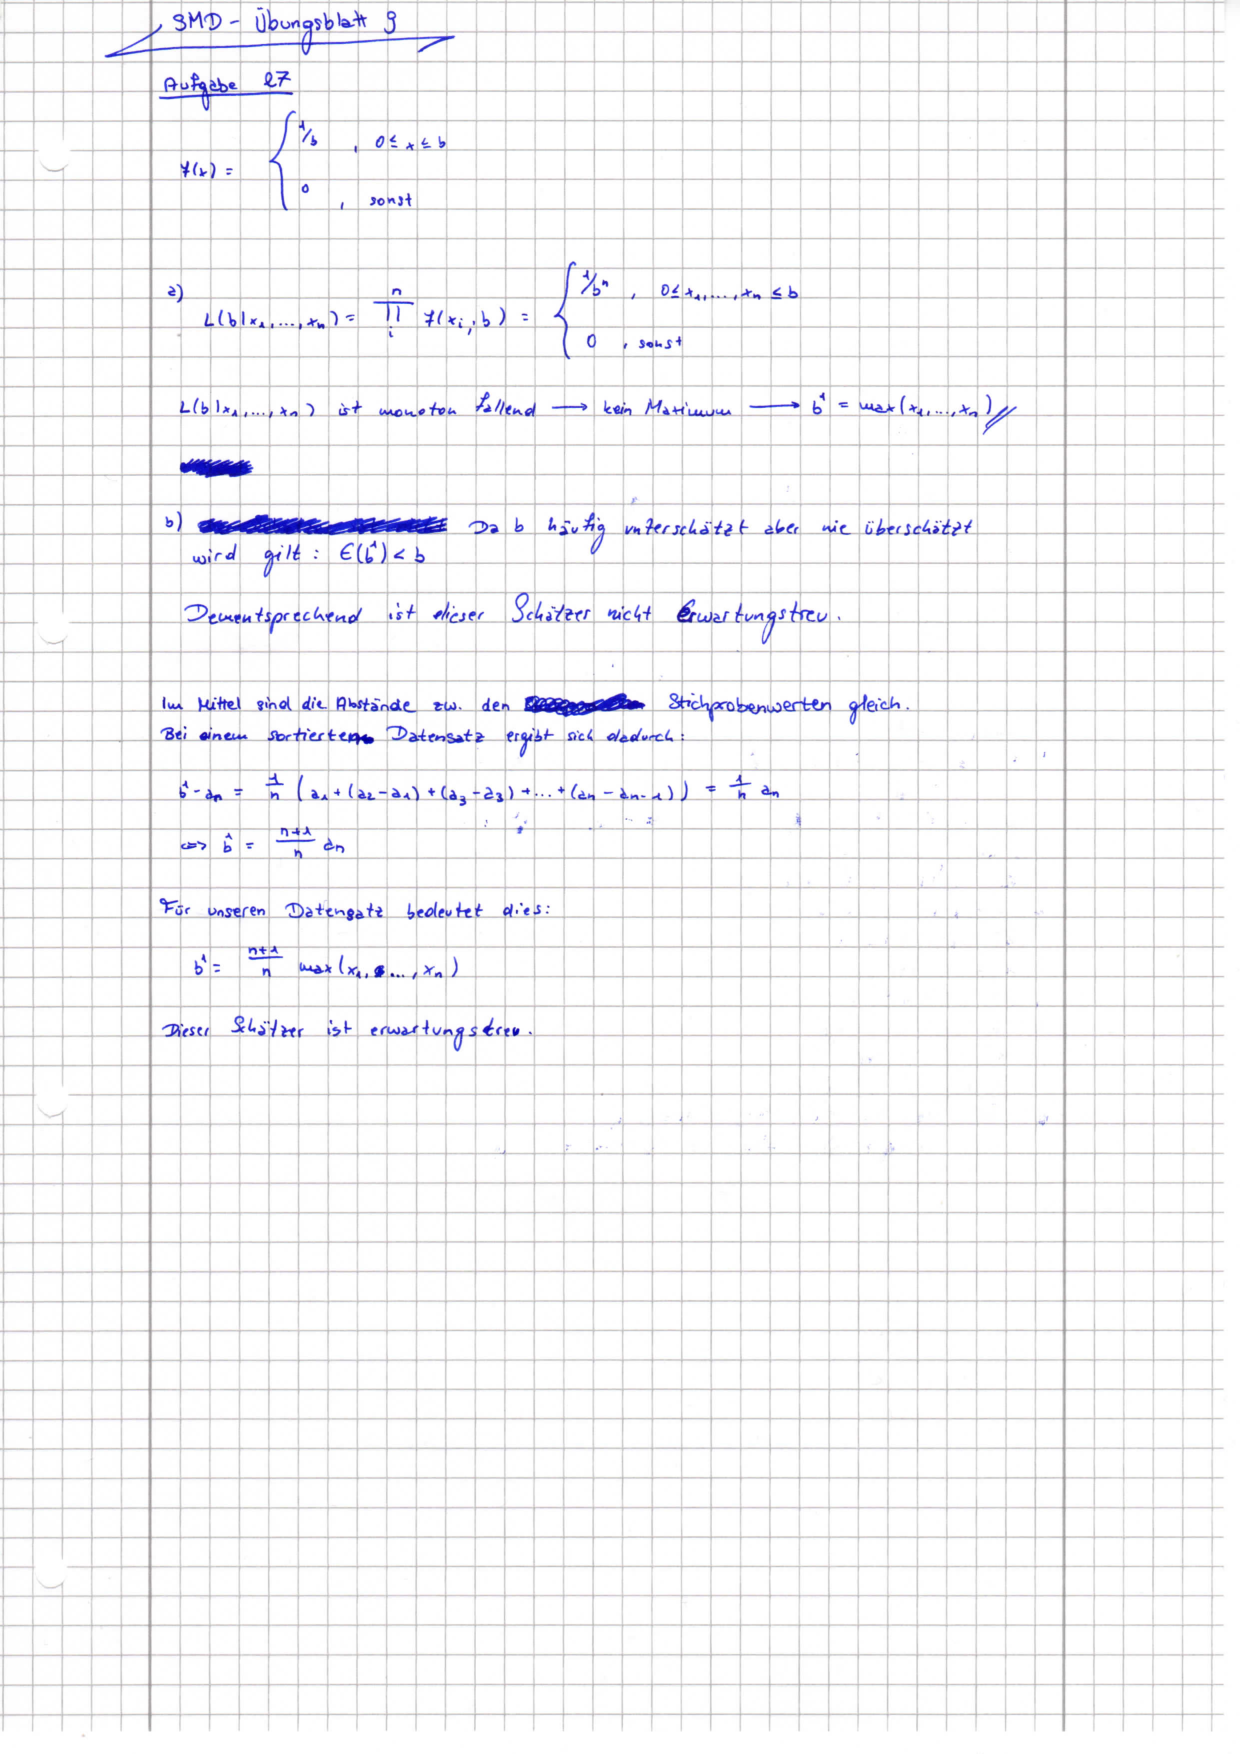
\includepdf[pages=-]{Aufgabe27/aufgabe27.pdf}
%\printbibliography{}


\end{document}
